\documentclass[openany,oneside,12pt]{book}
\usepackage{hyperref}
\usepackage{amsmath}
\usepackage[utf8]{inputenc}
\usepackage{tcolorbox}
\usepackage{listings}
\usepackage{listings-golang} % import this package after listings
\usepackage{color}
\usepackage{amssymb}
\usepackage{tikz}
\usetikzlibrary{positioning}
\lstset{
	language=Golang,
	aboveskip=3mm,
	belowskip=3mm,
	showstringspaces=false,
	columns=flexible,
	basicstyle={\small\ttfamily},
	numbers=none,
	numberstyle=\tiny\color{gray},
	keywordstyle=\color{blue},
	commentstyle=\color{red},
	stringstyle=\color{red},
	breaklines=true,
	breakatwhitespace=true,
	tabsize=3}
\title{MFree: An Explicit Meshfree Code for Non-Linear Solid Mechanics \\ release 0.1}
\date{2018 \\ October}
\author{Stephen Smith \\ Queen's University Belfast}



\newcommand*{\rttensor}[1]{\overline{\overline{#1}}}
\newcommand*{\rttensortwo}[1]{\ubar{\ubar{#1}}}

\raggedbottom
\begin{document}
\frontmatter
\vbox{
	\centering
		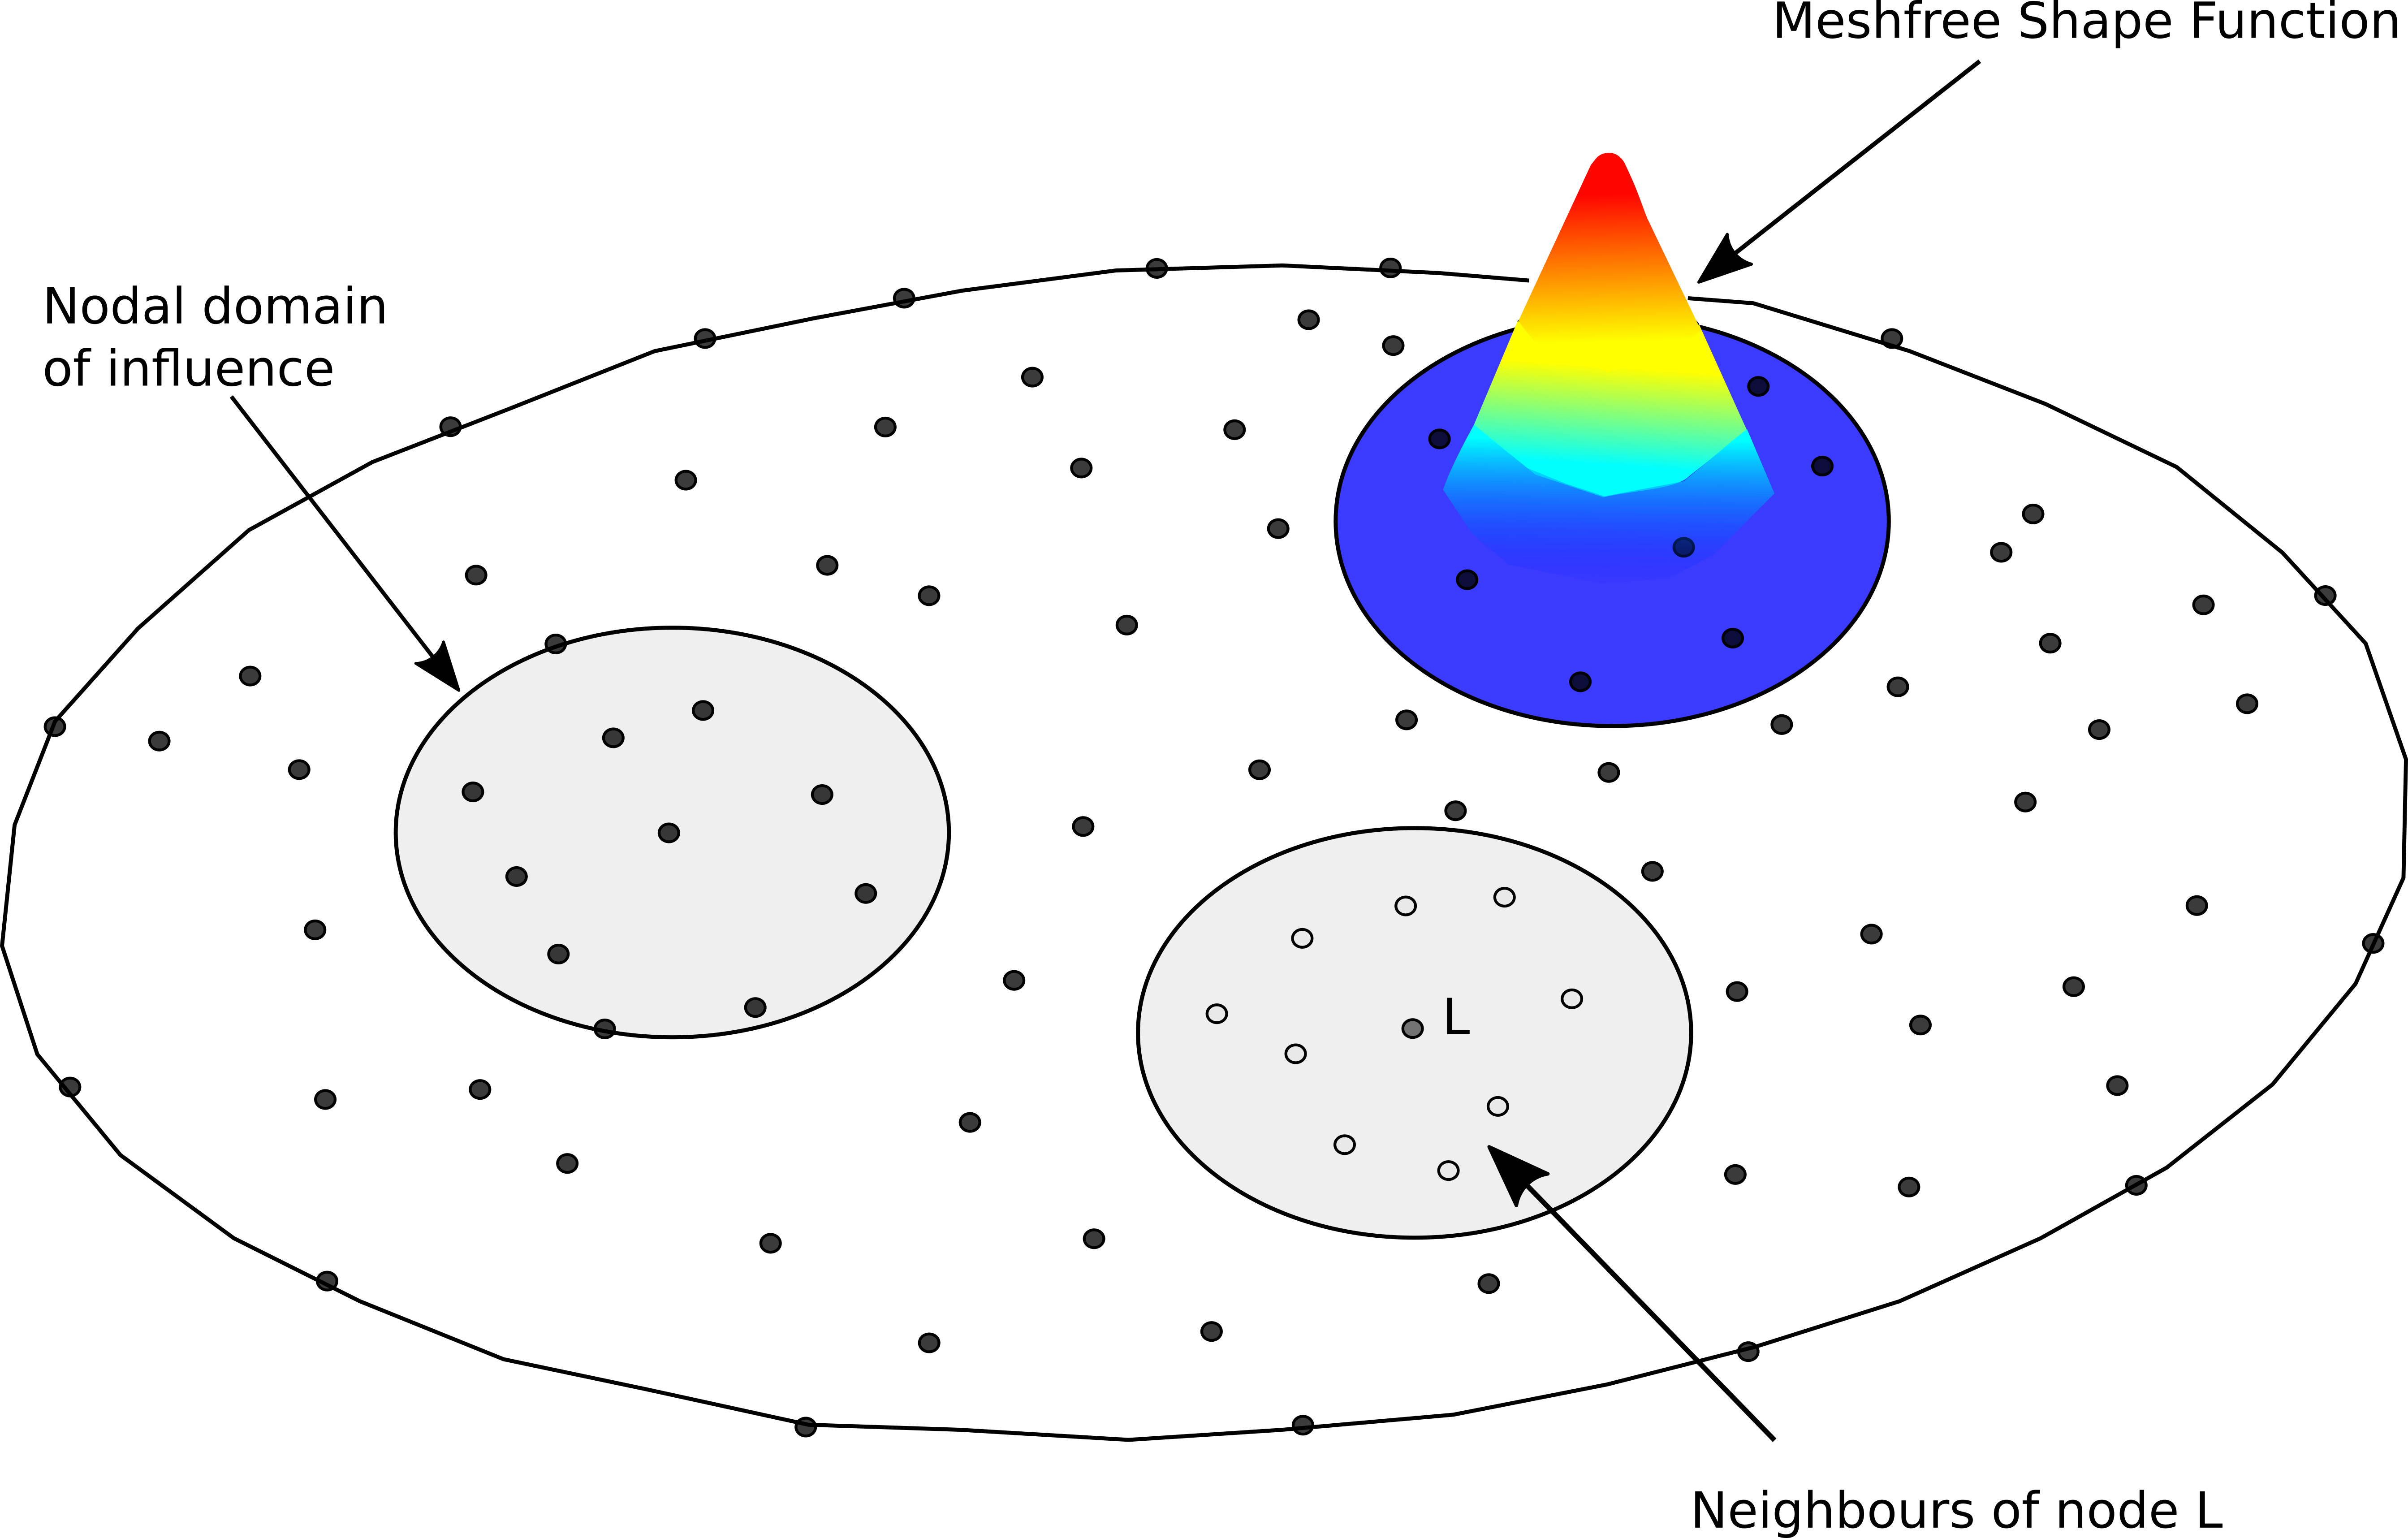
\includegraphics[width=0.9\textwidth,keepaspectratio]{MeshfreeDisc}
	\maketitle %this typesets the contents of \title, \author and \date
}
\tableofcontents
\mainmatter
\chapter{Introduction}
\section{MFree}
The Mfree libary is a framework developed in go-lang for mesh-free modelling in a research environment. It was developing during my PhD for application to stretch blow moulding a manufacturing technique used to produce polymer bottles. The main features of the code are the ability to simulate non-linear solid mechanics problems using an explicit solver. The use of the MFree library is intended to simplify the use of mesh-free methods within a research context, and further provide a learning resource for meshfree methods. 

To facilitate this goal, this manuscript has been created in order to describe the main features of this code. The code has been intended to be designed around the idea of the interaction between objects, similar to the object oriented style of programming, without the complexities of inheritance and polymorphism present in other langauges such as C++ and Java. Hence, it is the aim of this code is to provide a balance between a user friendly black-box (similar to Abaqus) and a tool for researchers within computational mechanics.

The go-lang langauge has been chosen as it provides inbuilt conncurncy along with a readability, and usability often not found in other high performance langauges (C, Fortran, C++).
\section{Overview}



\chapter{Theory}		
In order to understand how to use the library it is necessary to have an appreciation of the theory behind the application of meshfree methods to non-linear solid mechanics. This chapter explains the fundamental ideas of meshfree methods, and discretization of a continous problem in a discrete, and numerically solvable one. 
\section{Meshfree methods}
Meshfree methods were developed in the middle of the 1990's to overcome difficulties associated with the finite element method. The fundamental problem in meshfree or finite elements is to provide a set of approximation function (subject to a set of constraints) that can be used as an approximation space for the trial and test functions in the weak form of a partial different equation.  To illustrate this problem, consider the balance of linear momentum, cast in a Lagrangian(reference) form Eq. (\ref{Balance of linear momentum}). The intention in this manuscript is to use capital symbols to describe material coordinates, however often irregularities will exist between this intention and the result. 
\begin{equation}\label{Balance of linear momentum}
\text{GRAD} ~ P_{iJ} = \rho_0 \ddot{u_i}
\end{equation}
where $P$ is the first Piola-Kirchoff stress, $\rho_0$ the material density in the reference frame (typically $t=0$) and $\ddot{u}$ the acceleration. To complete the balance of linear moemntum boundary conditions must be specified. A boundary is called a displacemnt boundary, denoted $\Gamma_u$, if a displacement $u$ is prescribed on that boundary, likewise a similar defintion is present for the traction boundary, denoted $\Gamma_t$ The boundary conditions for Eq. (2.1) are typically given as:
\begin{equation}
u_i=\bar{u_i} ~~on ~~\Gamma_u
\end{equation}
\begin{equation}
P_{ij}N_j = \bar{T_i} ~~on ~~\Gamma_t
\end{equation}
Equation 2, subject to the boundary conditions (2.2,2.3) is often termed the strong form 

	
\begin{tcolorbox}
\textbf{Strong form of the momentum balance}
\begin{align*}
\text{GRAD} ~ P_{iJ} &= \rho_0 \ddot{u_i} &\text{Momentum Balance} \\
u_i&=\bar{u_i} ~~on ~~\Gamma_u &\text{Displacement condition} \\
P_{ij}N_j &= \bar{T_i} ~~on ~~\Gamma_t &\text{Traction condition}
\end{align*}
\end{tcolorbox}

\subsection*{Strong form to weak form }
To construct the weak form a test function $\delta u$ is introduced, which is assumed to be smooth enough up to the required order of the problem, and vanishes on the displacement boundary. The strong form, denoted $\mathcal{S}(u)$ of Box 1 is now cast into an alternate, but equivalent problem: 
\vspace{0.5cm}

\noindent\emph{Given a strong form $\mathcal{S}(u)$, find the trial dispalcemnt field $u(X,t)$ such that the following equation is satisfied }
\begin{equation}
\int{\delta u_i \cdot [GRAD ~P_{iJ} - \rho_0 \ddot{u}     ] d\Omega} = 0
\end{equation}
which is obtained from integrating the product of the strong form $S(u)$ and the test functions $\delta u$. Expanding (2.4) using the product rule of integration leads to the following form: 
\begin{equation}
\int{\big(\text{GRAD}~\delta u_i P_{iJ} + \delta u_i \rho_0 \ddot{u}_i \big) d\Omega     } - \int{\bar{T_i} \delta u_i d \Gamma_t} = 0
\end{equation}
This form of the equation can conveniently (for the sake of physical interpretation) be cast into the the principle of virtual work:
\begin{align}
\delta W &= \delta W^{int} - \delta W^{ext} + \delta W^{kin} 
\end{align}
Before summarising the derivation it is necessary to make a note on the definition of the trial and test functions. Firstly as mentioned above the test functions $\delta_u$ should vanish on the displacement boundary, and be continuous up to order required, which in the above form requires the existence of the first derivatives. With reference to this we define the space of functions $\mathcal{U}_0$ that satisfy these conditions:
\begin{equation}
\delta u(X) \in \mathcal{U}_0 ~~ \text{where} ~~ \mathcal{U}_0 = \{ \delta u(X) | \delta u(X) \in C^0(X), \delta u = 0 ~on~ \Gamma_u         \}
\end{equation}
In a similar manner the functions space for the trial functions $u(X,t)$ can be defined, with the condition that the displacemnt boundary conditions are satisfied. 
\begin{equation}
 u(X,t) \in \mathcal{U} ~~ \text{where} ~~ \mathcal{U} = \{u(X,t) | u(X,t) \in C^0(X), u(X,t) = \bar{u} ~on~ \Gamma_u         \}
\end{equation}
Combining these definitions with the principle of virtual work above leads to the complete problem, given by:
\begin{tcolorbox}
	\textbf{Principle of virtual work (Weak form)}
	Find the trial functions u(X,t) such that for any admissible (member of $\mathcal{U}_0$) virtual displacement $\delta u$ the virtual work $\delta W $ is zero.
	\begin{equation*}
	\delta W = \delta W^{int} - \delta W^{ext} + \delta W^{kin} 
	\end{equation*}
	where 
	\begin{align*}
	\delta W^{int} &= \int{\text{GRAD}~\delta u_i P_{iJ}d \Omega} \\
	\delta W^{ext} &=  \int{\bar{T_i} \delta u_i} d \Gamma_t \\
	\delta W^{kin} &= \int{\delta u_i \rho_0 \ddot{u}_i d \Omega}
	\end{align*}
\end{tcolorbox}
\subsection*{Discretization}
The weak form in Box 2 still requires the determination of the continuous function $u(X,t)$ which in most cases will be impossible. A set of discrete equations can be developed by considering an approximation of the displacements, which in its most general form: \emph{Given a set of data points $X \in \mathcal{R}^d$, with nodal values $u_d$}. Any approximation scheme is subject to a minimum of two constraints in order to be applied to the virtual work statement above:
\begin{tcolorbox}
\textbf{	Shape function requirements}
	\begin{enumerate}
		\item The shape functions should be able to reproduce a constant field
		\begin{equation*}
		\implies \sum_I \phi_I = 1
		\end{equation*}
		\item In order to ensure first order convergence the shape functions should be able to reproduce a polynomial
		\begin{equation*}
		\implies \sum_I \phi_I x_{kI} = x_k ~~ for~k=1,2,3
		\end{equation*}
	\end{enumerate}
\end{tcolorbox}
\noindent This leads to the following form

\begin{equation}
u(X,t) = \sum_I^N \phi_I(X) u_{Ii}(t)
\end{equation}
and the derivative by:
\begin{equation}
u(X,t),_J = \sum_I^N \phi_I(X),_J u_{Ii}(t) ~~where~j = 1,..,n_d
\end{equation}
The construction of the shape functions $\phi_I$ is dependent on the method used. If the data points X are arranged into convex polygons, then the shape functions coincide with those used in the finite element method. However, this predefined computational mesh can create issues in large deformation, which lead to the develop of meshfree approximation methods. In this case an arbitrary, but local support is assigned to each node Fig. 1. The simplest shape function that can be constructed for this domain is the shepard function, defined by a ratio of the weight functions
\begin{equation}
\phi_i = \frac{\omega_a (x; x-x_i)}{\sum_j^n \omega_a(x;x-x_j)} 
\end{equation}
which clearly satisfies the first condition (constant reproduction) as
\begin{equation}
\sum_i \phi_i = \frac{\sum_i^n\omega_a (x; x-x_i)}{\sum_j^n \omega_a(x;x-x_j)} = 1
\end{equation}
However, in order to satisfy the linear reproducing conditions an additional enrichment term is required. Consider the general form of the meshfree aporixmation given by 
\begin{equation}
u^h(x) = \sum_i^n C_i(x) \Gamma_i(x)
\end{equation}
.........



\subsubsection*{Probabilistic Approach}
The approach above for developing meshfree shape functions leads to one drawback, the shape functions no longer interpolate data, which presents problems in implementing boundary conditions. In order to fix this issue a probablistic approach to mesh-free shape functions was developed by Ortiz \cite{}, known as the MAXENT scheme. In this approach the problem is: \emph{Given a of mutally independent discrete events $e_1,e_2,...,e_n$, that occur with probabilities $p_1,p_2,...,p_n$}

\begin{tcolorbox}
\textbf{MAXENT Construction:}
Minimise the convex potential functions $F(\lambda_1,\lambda_2) = log(\sum_I e^{-\lambda_1 \tilde{x}_i - \lambda_2 \tilde{y}_i})$ Method: Assume that the solution $\lambda^k$ at the $kth$ iteration is given, then the minimisation problem can be expanded using a taylor series
\begin{equation*}
0 = \mathcal{R}(\lambda^k) + \nabla \nabla F(x) \Delta \lambda^k
\end{equation*}
Which is a Newton-Raphson scheme, shown pictorially in figure 2.
\end{tcolorbox}
\section{Constitutive Modelling}

\chapter{Design}
\section{Domain}

\subsubsection*{Overview}
The domain package is intended to hold together the geometric details of the problem, i.e the nodes, the intergration cells and the degrees of freedom attached to the domain. From this other packages will refrence this domain, such as the meshfree packaage, which builds the meshfree domain, and the integration package. At present there are two ways to build a domain, manually by adding nodes to a domain object, or more simply by providing a planar-straight line graph (PLSG) to the domain constructor, given by:
\begin{tcolorbox}
\begin{lstlisting}
domain := domain.DomainNew(fileName string, options string, dim int, global_coordinate coordinateSystem)
\end{lstlisting}
\end{tcolorbox}

Where $fileName$ is the name of the PLSG, $options$ provides a set of rules the mesh, and voronoi generator, see \url{https://www.cs.cmu.edu/~quake/triangle.html} for a description. The variable $dim$ ensures that correct number of degrees of freedom(DOFs) will be set. The coordinate system can be generated using the following function (for Cartesian coordinates),
\begin{lstlisting}
globalCS := coordinatesystem.CreateCartesian()
\end{lstlisting}
axisymmetric (cylindrical coordinates) are also supported. This function will construct the nodes, the degrees of freedom (assuming they are all free to start with) and the Voronoi diagram, which is used in the stabalised nodal integration scheme (SCNI).

\subsubsection*{Public functions}

\subsubsection*{Private functions}	
\chapter{Furture Plans}
\chapter{Area of Improvements}	
As the matrix library (gonum) is based off the blas libaries the performance for smaller domains is expected to be poor due to the overhead of calling the blas routines. Therefore it may be best to rediesng the shape function library.
\chapter{Acknowledgements}
The following packages have been used in this project
\end{document}